\documentclass[letterpaper]{article}
\usepackage[utf8]{inputenc}
\usepackage{pgf, tikz}
\usepackage{pgfplots}
\usetikzlibrary{arrows, automata}
\usetikzlibrary{graphs, graphs.standard}
\usepackage{amsmath}
\tikzset{
  common/.style={draw,name=#1,node contents={},inner sep=0,minimum size=3},
  disc/.style={circle,common=#1},
  square/.style={rectangle,common={#1}},
}

\begin{document}

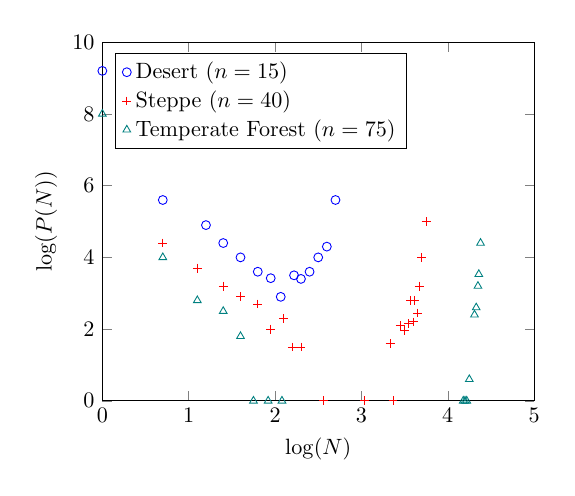
\begin{tikzpicture}[scale = 0.8]
\begin{axis}[
  only marks,                    % no lines
  xmin=0, xmax=5,              % x-axis limits
  ymin=0, ymax=10,              % y-axis limits
  xlabel={$\log(N)$},      % x-axis label
  ylabel={$\log(P(N))$},            % y-axis label
  legend pos=north west,         % legend position on plot
  legend cell align=left,        % text alignment within legend
  samples=200,                   % plot 200 samples
]
  \addplot[mark=o,blue] coordinates {
            (0,9.2)
            (0.7,5.6)
            (1.2,4.9)
            (1.4,4.4)
            (1.6,4)
            (1.8,3.6)
            (1.95,3.42)
            (2.066,2.9)
            (2.22,3.5)
            (2.3,3.4)
            (2.4,3.6)
            (2.5,4)
            (2.6,4.3)
            (2.7,5.6)         
  }; % ...
  \addlegendentry{Desert ($n=15$)};
  \addplot[mark=+,red] coordinates {
            (0.7,4.4)
            (1.1,3.7)
            (1.4,3.2)
            (1.6,2.9)
            (1.8,2.7)
            (1.95,2)
            (2.1,2.3)
            (2.2,1.5)
            (2.3,1.5)
            (2.566,0)
            (3.033,0)
            (3.333,1.6)
            (3.366,0)
            (3.45,2.1)
            (3.5,1.95)
            (3.55,2.15)
            (3.57,2.8)
            (3.62,2.8)
            (3.6,2.2)
            (3.65,2.45)
            (3.67,3.2)
            (3.7,4)
            (3.75,5)
  };
  \addlegendentry{Steppe ($n=40$)};
  \addplot[mark=triangle,teal] coordinates {
            (0,8)
            (0.7,4)
            (1.1,2.8)
            (1.4,2.5)
            (1.6,1.8)
            (1.75, 0)
            (1.92,0)
            (2.08,0)
            (4.18,0)
            (4.2,0)
            (4.22,0)
            (4.25,0.6)
            (4.31,2.4)
            (4.33,2.6)
            (4.35,3.2)
            (4.36,3.53)
            (4.38,4.4)
  }; % add the first plot
  \addlegendentry{Temperate Forest ($n=75$)}; % add the first plot's legend entry
\end{axis}
\end{tikzpicture}

\end{document}